\chapter{User Study}
\label{userStudy}

\section{Structure} We created a multi-wave user study to examine the effectiveness of different parts of our program. 

In the first phase, we had \uniqueUsersPhaseOneUserStudy people record over \numResponsesPhaseOneUserStudy different phrases, to see how they pronouced them.  This phase served two purposes: one, to gather recordings for the second phase, and two, to see if our phonemic transcriptions were valid.  

In the second phase, we took \recordingsPhaseTwoUserStudy recordings of oronyms from phase one, and gathered \numTranscriptionsPerRecordingPhaseTwoUserStudy transcriptions for each recording, resulting in a total of \numResponsesPhaseTwoUserStudy transcriptions. These transcriptions were provided by \uniqueUsersPhaseTwoUserStudy unique users ( \uniqueUsersPhaseTwoUserStudyUSA from the United States).  We then compared the transcriptions of the recorded oronym phrases to the calculated oronyms for the original root phrase.

\section{User Sampling Population}
We drew our test subjects from a pool of Amazon Mechanical Turk workers (hired for \$ 0.02 to \$ 0.10 per task) and, for part of phase 1, volunteers from Reddit.com \cite{redditAssistance} \cite{redditRecordThis}. 

Amazon Mechanical Turk is an online crowdsourcing service where requesters can hire workers to complete Human Intelligence Tasks, or HITs.  The efficacy of using Mechanical Turk for user studies has been widely studied in academia, and specifically proven in the linguistic community \cite{sprouse_validation_2011}.


\section{Methodology}

\subsection{First Phase: Recitation}
\label{subsection:firstWaveUserStudy}
In this wave of the user study, we used a combination of \uniqueUsersPhaseOneUserStudy Mechanical Turk workers (hired for \$ 0.10 per task) to record \numResponsesPhaseOneUserStudy different phrases.  These phrases were oronyms of one of two phrases: phrase A, ``a nice cold hour" or phrase B, `` fourth rye to".  To keep track of the phrases, we assigned each phrase an phraseID, built off of the phrase letter, phrase length, and phrase text.    We gave Mechanical Turk workers three minutes to record each phrase and email it to us with the phrase identifier in the subject of the email. The number of recordings per phrase, along with their identifiers, can be seen in table ~\ref{table:phrasesRecorded}.


\begin{center}

%\begin{table}

\begin{longtable}{|c|c|c|}
\caption[Phrases Recorded]{Here are the phrases we recorded, how many times they were recorded, and the identifiers we used for each phrase}
\label{table:phrasesRecorded} 

\hline 
orthoPhrase & numRecordings & phraseID \\
\endfirsthead

\multicolumn{3}{c}%
{{\bfseries \tablename\ \thetable{} -- continued from previous page}} \\
\hline
orthoPhrase & numRecordings & phraseID \\
\endhead


\hline \multicolumn{3}{|r|}{{Continued on next page}} \\ \hline
\endfoot

\hline \hline
\endlastfoot

\hline
a nice cold our   & 3 & A.17.51    a nice cold our  \\
\hline
an ice cold our   & 2 & A.17.135    an ice cold our  \\
\hline 
a nye scold our   & 2 & A.17.69    a nye scold our  \\
\hline 
ah nye scold our   & 2 & A.18.109    ah nye scold our  \\
\hline 
an eye scold our   & 2 & A.18.125    an eye scold our  \\
\hline 
on aye scold our   & 2 & A.18.267    on aye scold our  \\
\hline 
a nigh scold our   & 2 & A.18.65    a nigh scold our  \\
\hline 
a nye skol dower   & 2 & A.18.71    a nye skol dower  \\
\hline 
an aye skol dower   & 2 & A.19.119    an aye skol dower  \\
\hline 
an eye skol dower   & 2 & A.19.127    an eye skol dower  \\
\hline 
an ice coal dower   & 2 & A.19.133    an ice coal dower  \\
\hline 
eh nice coal dower   & 2 & A.20.159    eh nice coal dower  \\
\hline 
ah nice coal dower   & 2 & A.20.89    ah nice coal dower  \\
\hline 
fourth wry to   & 2 & B.15.19    fourth wry to  \\
\hline 
fourth wry too   & 2 & B.16.20    fourth wry too  \\
\hline 
forth right ooh   & 2 & B.17.1    forth right ooh  \\
\hline 
fourth rite ooh   & 2 & B.17.13    fourth rite ooh  \\
\hline 
forth wright ooh   & 2 & B.18.6    forth wright ooh  \\
\hline 
on i scold our   & 1 & A.16.279    on i scold our  \\
\hline 
an i scold hour   & 1 & A.17.128    an i scold hour  \\
\hline 
an i skol dower   & 1 & A.17.131    an i skol dower  \\
\hline 
an ice-cold our   & 1 & A.17.141    an ice-cold our  \\
\hline 
on i scold hour   & 1 & A.17.278    on i scold hour  \\
\hline 
on i skol dower   & 1 & A.17.281    on i skol dower  \\
\hline 
an aye scold our   & 1 & A.18.117    an aye scold our  \\
\hline 
an ice cold hour   & 1 & A.18.134    an ice cold hour  \\
\hline 
an ice-cold hour   & 1 & A.18.140    an ice-cold hour  \\
\hline 
eh nye scold our   & 1 & A.18.179    eh nye scold our  \\
\hline 
on eye scold our   & 1 & A.18.275    on eye scold our  \\
\hline 
on ice cold hour   & 1 & A.18.284    on ice cold hour  \\
\hline 
on ice-cold hour   & 1 & A.18.290    on ice-cold hour  \\
\hline 
a nye scold hour   & 1 & A.18.68    a nye scold hour  \\
\hline 
ah nice cold our   & 1 & A.18.91    ah nice cold our  \\
\hline 
ah nigh scold our   & 1 & A.19.105    ah nigh scold our  \\
\hline 
ah nye scold hour   & 1 & A.19.108    ah nye scold hour  \\
\hline 
ah nye skol dower   & 1 & A.19.111    ah nye skol dower  \\
\hline 
an aye scold hour   & 1 & A.19.116    an aye scold hour  \\
\hline 
an ice kohl dower   & 1 & A.19.139    an ice kohl dower  \\
\hline 
eh nice cold hour   & 1 & A.19.160    eh nice cold hour  \\
\hline 
eh nigh scold our   & 1 & A.19.175    eh nigh scold our  \\
\hline 
eh nye skol dower   & 1 & A.19.181    eh nye skol dower  \\
\hline 
on aye skol dower   & 1 & A.19.269    on aye skol dower  \\
\hline 
on eye scold hour   & 1 & A.19.274    on eye scold hour  \\
\hline 
on ice coal dower   & 1 & A.19.283    on ice coal dower  \\
\hline 
on ice kohl dower   & 1 & A.19.289    on ice kohl dower  \\
\hline 
a nice coal dower   & 1 & A.19.49    a nice coal dower  \\
\hline 
a nigh scold hour   & 1 & A.19.64    a nigh scold hour  \\
\hline 
ah nice cold hour   & 1 & A.19.90    ah nice cold hour  \\
\hline 
eh nice cole dower   & 1 & A.20.163    eh nice cole dower  \\
\hline 
eh nigh scold hour   & 1 & A.20.174    eh nigh scold hour  \\
\hline 
eh nigh skol dower   & 1 & A.20.177    eh nigh skol dower  \\
\hline 
ah nice cole dower   & 1 & A.20.93    ah nice cole dower  \\
\hline 
ah nice kohl dower   & 1 & A.20.95    ah nice kohl dower  \\
\hline 
forth wry two   & 1 & B.15.10    forth wry two  \\
\hline 
forth rye two   & 1 & B.15.5    forth rye two  \\
\hline 
forth write ooh   & 1 & B.17.7    forth write ooh  \\
\hline 
fourth right ooh   & 1 & B.18.12    fourth right ooh  \\
\hline 
fourth wright ooh   & 1 & B.19.17    fourth wright ooh  \\
\hline

\end{longtable}

%\end{table}
\end{center}

We then transcribed the phonetics of each of the recording in SAMPA by ear.  In a stunning example of a use case for our project, we discovered that we had unintentionally included some phrases for recordings were not deterministically phonetically parsible, meaning that our oronyms had multiple pronunciations, not all of which mapped back to the original phrase.  For example, the orthographic word ``a" can be interpreted as the phoneme `A', and that `A' phoneme can be combined with the subsequent `n' phoneme from the word ``nice" to create the SAMPA sequence `An'.  That being said, this fit with our model, and we found no unexpected anomalies when comparing our transcriptions to the expected SAMPA spellings of each phrase.




\subsection{Recording Sample Pool}
\label{subsection:recordingSamplePool}
We had originally intended to use all the phase one recordings in phase two, but eventually had to discard all but \recordingsPhaseTwoUserStudy of the recordings for various reasons, the most common being that the recording was too loud and we wanted to spare our user's ears, or the person recording left excessive amounts of space between words that overly-segmented the phrase.  The recordings for the ``fourth rye to" oronyms were all unusable for phase two, because our users tended to insert exclamation points any time they said ``ooh" or ``too", overloading their microphones or over-segmenting the phrase.

All \recordingsPhaseTwoUserStudy recordings we used were oronyms for the phrase ``a nice cold hour", and were recorded by one man with remarkably smooth diction from the midwest, which made him the best approximation we could get for a General American accent.

\subsection{Second Wave: Transcription}
\label{subsection:secondWaveUserStudy}

We hired \uniqueUsersPhaseTwoUserStudy unique Mechanical Turk workers to transcribe our oronym recordings for \$ 0.02 to \$ 0.03 per transcription.  Each of the \recordingsPhaseTwoUserStudy recordings was transcribed \numTranscriptionsPerRecordingPhaseTwoUserStudy times, resulting in a total of \numResponsesPhaseTwoUserStudy transcriptions. These transcriptions were provided by \uniqueUsersPhaseTwoUserStudy unique users ( \uniqueUsersPhaseTwoUserStudyUSA from the United States). In addition to transcribing the recording, in each task, the worker was asked what country they were from. We did this to help differentiate native American English speakers from non-native speakers.

\begin{figure}
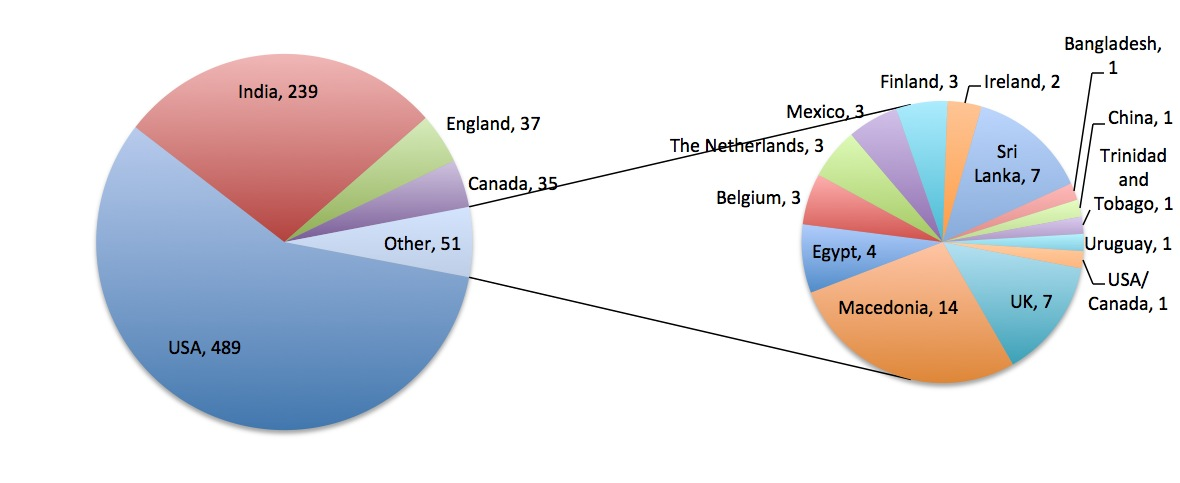
\includegraphics[width=150mm]{responsesPerCountry.jpg}
\captionfonts
\caption[Responses Per Country]{ Our user study primarily polled people from the United States and India, as can be seen by the number of responses originating from each country. }
\label{fig:responsesPerCountry}
\end{figure}

\begin{table}
\begin{center}

\begin{tabular}{|c|c|c|}
\hline 
Response By Country   &   Num Responses   \\ \hline
USA   &   489   \\ \hline
India   &   239   \\ \hline
England   &   37   \\ \hline
Canada   &   35   \\ \hline
UK   &   7   \\ \hline
Macedonia   &   14   \\ \hline
Egypt   &   4   \\ \hline
Belgium   &   3   \\ \hline
The Netherlands   &   3   \\ \hline
Mexico   &   3   \\ \hline
Finland   &   3   \\ \hline
Ireland   &   2   \\ \hline
Sri Lanka   &   7   \\ \hline
Bangladesh   &   1   \\ \hline
China   &   1   \\ \hline
Trinidad and Tobago   &   1   \\ \hline
Uruguay   &   1   \\ \hline
USA/Canada   &   1   \\ \hline
\end{tabular}

\captionfonts
\caption[Countries and responses]{ Here's a table with the number of responses per country}
\label{table:countryTally}
\end{center}
\end{table}

